%
% File acl2018.tex
%
%% Based on the style files for ACL-2017, with some changes, which were, in turn,
%% Based on the style files for ACL-2015, with some improvements
%%  taken from the NAACL-2016 style
%% Based on the style files for ACL-2014, which were, in turn,
%% based on ACL-2013, ACL-2012, ACL-2011, ACL-2010, ACL-IJCNLP-2009,
%% EACL-2009, IJCNLP-2008...
%% Based on the style files for EACL 2006 by 
%%e.agirre@ehu.es or Sergi.Balari@uab.es
%% and that of ACL 08 by Joakim Nivre and Noah Smith

\documentclass[11pt,a4paper]{article}
\usepackage[hyperref]{acl2018}
\usepackage{times}
\usepackage{latexsym}
\usepackage{graphicx}
\graphicspath{ {images/} }

\usepackage{url}

\definecolor{customGreen}{RGB}{61, 219, 30}
\definecolor{customRed}{RGB}{229, 18, 18}

% this is needed due to the at-the-moment-still-empty bbl file. Otherweise we have an error
\makeatletter
\def\endthebibliography{%
	\def\@noitemerr{\@latex@warning{Empty `thebibliography' environment}}%
	\endlist
}
%source: https://tex.stackexchange.com/questions/350907/error-latex-error-somethings-wrong-perhaps-a-missing-item/350921
\makeatother
\label{key}

\aclfinalcopy % Uncomment this line for the final submission
%\def\aclpaperid{***} %  Enter the acl Paper ID here

%\setlength\titlebox{5cm}
% You can expand the titlebox if you need extra space
% to show all the authors. Please do not make the titlebox
% smaller than 5cm (the original size); we will check this
% in the camera-ready version and ask you to change it back.

\newcommand\BibTeX{B{\sc ib}\TeX}

\title{Named Entity Recognition in the \textit{Regesta Imperii} \\-\\ Person and Location Names in the late Middle Ages}

\author{Jana H{\"a}n{\ss}ler \\
  Technische Universit{\"a}t Darmstadt  \\
  Institut f{\"u}r Sprach- und Literaturwissenschaft \\
  Computer Applications in Linguistics\\
  Dr. Sabine Bartsch
}

\date{}

\begin{document}
\maketitle
\begin{abstract}
	Recognizing entities in texts can be done automatically. In the study at hand, a model for Named Entity Recognition in a special corpus, the Regesta Imperii, is trained. The performance evaluation of the given tags for person names, titles, and location names reveals weaknesses which are probably caused by an insufficient amount of training data. Nevertheless, an analysis of names in the late Middle Ages is made by means of the tagger's results.
\end{abstract}

\section{Introduction}
\label{cha:intro}
Jurafsky and Martin \cite{jurafsky_speech_2017} define Named Entity Recognition (NER) as the task of "[...] finding spans of text that constitute proper names and then classifying the entities being referred to according to their type." A more precise definition of NER is the one of Bartsch and Weber \cite{bartsch_linguisticsweb:tutorials:linguistics_tutorials:automaticannotation:stanford_ner_2015}. They give an overview over the purpose and the usage of NER:

\begin{quote}
The detection of named entities can be useful for computational analysis of literary texts. Questions concerning the narrative structure can be answered: Which characters are introduced in which part of the text, which places are mentioned? Moreover, named entity recognition is a subtask in the field of information extraction. It is an important component if you are dealing with question answering or co-reference resolution.6
\end{quote}

The topic of and the interest in NER is more up to date than ever before. As the quantity of (digital) texts increases massively in the present age, science and economics seek to analyze these masses of text. In a previous study\footnote{For further details the interested reader may see H{\"a}n{\ss}ler (2016) \textit{Hausarbeit NER – theoretisch} – a paper which introduces and compares these two types of NER with one another.}, two tools for the task of NER – the \textit{Stanford Named Entity Recognizer} (SNER) and the application \textit{ANNIE} with a German gazetteer in \textit{GATE} – were used and tested. As a result of this study, neither the one nor the other worked satisfyingly. For this reason, this paper presents the training of a named entity recognizer, which, in the end, is supposed to yield better results than the ready-made ones. The aim of this study is to do NER for person and location names in the \textit{Regesta Imperii}\footnote{The project \textit{Regesta Imperii} will be introduced in chapter 3 – The Corpus.} (RI). If the tagger does not yield better results than those from the previous study, suggestions for its improvement shall be derived from the study at hand. The idea is, however, to test borders of feasibility of the SNER instead of programming a perfectly working NE-tagger.

One kind of purpose of NER and of the research presented in this paper (and in general, too,) is to contribute to a faster recognition of names in a big corpus and therefore to a better understanding as well as further processing of the data (in the RI project). Entities – here person and location names – in the RI shall automatically be recognized and tagged. The basic idea here is that these automatically tagged entities can then be examined and further processed. From a linguistic point of view, the structure of the found entities, especially of the person names, is interesting. What do names in the RI look like? How are they represented in this special corpus? Furthermore, the search function of the \textit{RI online} and accordingly the data provision for the scientific user may be improved by the present work. 

After presenting the corpus and its challenging characteristics in chapter \ref{cha:corpus}, chapter \ref{cha:tool} depicts how the training of a NER-model was carried out, what is needed for its accomplishment, and gives short annotation guidelines. The last chapter attends to the concrete NER task and its evaluation. Furthermore, chapter \ref{cha:results} takes a closer historic-cultural look at the recognized person names and their linguistic appearance.



\section{The Corpus}
\label{cha:corpus}
\subsection{The Project Regesta Imperii}
The corpus being under examination in this study is the texts of the project \textit{Regesta Imperii} (RI). It is a long-term project of three academies; the \textit{Academy of Sciences and Literature | Mainz}, the \textit{Austrian Academy of Sciences} and the \textit{Berlin-Brandenburg Academy of Sciences and Humanities}. In 1829, the Frankfurt city librarian Johann Friedrich B{\"o}hmer began with the collection of imperial documents, which – actually planned as groundwork for the \textit{Monumenta Germaniae Historica} – soon developed into an independent fundamental work (cf. Webseite der Regesta Imperii, Akademie der Wissenschaften und der Literatur; henceforce referred to as RIAdW; /unternehmen\footnote{\url{http://www.regesta-imperii.de/unternehmen.html}.}). The whole RI collection of regestas is subdivided into 14 sections, from Carolingians to Maximilan I. (ca. 751-1519). "The REGESTA IMPERII (RI) chronologically record all activities evidenced by charters and other sources of the Roman-German kings and emperors from the Carolingians up to Maximilian I (ca. 751-1519) as well as of the propes of the early Middle Ages and High Middle Ages in form of German ‘Regesten’ (abstracts)." (RIAdW\footnote{\url{http://www.regesta-imperii.de/en/research.html}.})

Regestas, in general, are short texts about documents; the RI regestas are short texts about medieval emperor documents. "A regesta sums up the essential content of a document in modern German and, moreover, offers statements about transmission and research state." (RIAdW\footnote{\url{http://www.regesta-imperii.de/unternehmen/videopraesentation.html}.}) The structure of each regesta is its text, the transmission and commentary as well as date and place of issue (RIAdW\footnote{\url{http://www.regesta-imperii.de/unternehmen/ri-online.html}.}). Currently (effective April 14, 2018), there are 90 printed volumes and 182.315 regesta online available as full text records via REST API (RIAdW\footnote{\url{http://www.regesta-imperii.de/en/daten.html}.}) in the RI Database which is licensed under a CC-BY 4.0 International\footnote{\url{https://creativecommons.org/licenses/by/4.0/}.} license.

\subsection{Challenges of the Corpus}
Bartsch and Weber \cite{bartsch_linguisticsweb:tutorials:linguistics_tutorials:automaticannotation:stanford_ner_2015} define entities as "[...] elements having a distinct, separate existence. These phrases contain, for instance, the names of persons, organizations, locations, times and quantities." From the viewpoint of linguistics, the regesta texts and its entities are interesting, but they also pose several challenges on the NE tagger.

As a first challenge, Benikova et al. \cite{benikova_nosta-d_nodate} state that German is difficult for NER (in comparison to English e.g.) because not only proper names are capitalized but also nouns. The RI are mostly written in German language. Some regesta texts may contain Latin or French passages. Secondly, many abbreviations in the corpus\footnote{Only the summary of the regesta document content is relevant.} may pose a difficulty for the NER process. \textit{König Friedrich}, for instance, usually is abbreviated as \textit{Kg. F.}, many other titles, too. Especially since the CRF classifier uses the word sequences in order to ‘learn’ how to tag entities, this might problematic. Usually, person and location names can be differentiated and extracted by NER systems. However, as the previous study and the examination of the \textit{Kumuliertes Register der bislang erschienenen Hefte. Regesten Kaiser Friedrichs III. (1440-1493)} \cite{rubsamen_accumulated_nodate} of all names and locations reveals, indications of person names often come along with a location name. In other words, many person names overlap with a location name. This is aggravated by the fact that titles, too, overlap with person names.

\section{The Tool}
\label{cha:tool}
\subsection{Training a Model}
The tool used in this study - or rather a component of it, namely its classifier - is the \textit{Stanford Named Entity Recognizer}. Because the pre-trained SNER-model did not yield satisfying results as shown in the previous study, it was the aim of the study at hand to improve the SNER-model or rather to train an own model for this special corpus.

For the training of an own model, Stanford offers a vague documentation\footnote{\url{https://nlp.stanford.edu/software/crf-faq.html\#a}.}. The process basically is a triad. In a first step, training data needs to be built. This "training data needs to be in tab-separated columns, with minimally the word tokens in one column and the class labels in another column." To give a limit to the number of texts worked with, a fraction of one volume - \textit{[RI XIII] H. 14 - Friedrich III., N{\"u}rnberg 1 (1440-1449)} - was chosen for this project; 21 of the entries (3115 tokens) from \textit{Heft 14 – Friedrich III., N{\"u}rnberg (1440-1149)} were 1) tagged with O (default value) by a \textit{Python} script\footnote{The script can be found in the GitHub repository \url{https://github.com/JanaHae/CAL}.} and 2) manually NE-tagged and served as training data.\footnote{The labeled training data can be found in the GitHub repository \url{https://github.com/JanaHae/CAL}.} The second step in the training process was to actually train the model. Therefore, a properties file\footnote{The properties file can be found in the GitHub repository \url{https://github.com/JanaHae/CAL}.} was created.

Via the \textit{Windows PowerShell} and the command in figure \ref{fig:TrainingCommand} the training process is started.
\begin{figure}[h]
	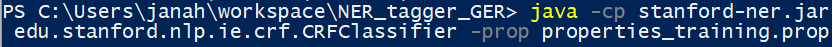
\includegraphics[scale=0.437]{command_training}
	\centering
	\caption{Command for Training}
	\label{fig:TrainingCommand}
\end{figure}

The classifier behind the SNER is a Conditional Random Field (CRF) classifier. While other models predict a tag only based on a single word, a CRF classifier also takes important pieces of information from the text - sequential data - to compute a probability of the output; it also considers the "neighboring" words. The NE tag with the highest probability is then applied. In a third step, the trained model was applied to the test data which consisted of 67 regesta texts from \textit{Heft 14 – Friedrich III., N{\"u}rnberg (1440-1149)}. This test file also had to be tokenized and labeled with the default value before applying the model to it.
\begin{figure}[h]
	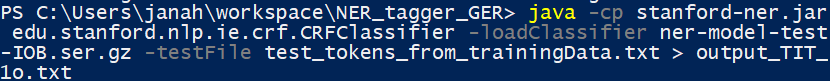
\includegraphics[scale=0.437]{command_testing}
	\centering
	\caption{Command for Testing}
	\label{fig:TestingCommand}
\end{figure}

The tagged data was outputted to the folder in which the model was saved.

\subsection{Annotation Guidelines}
This section gives a short overview of the guidelines which determined the annotation of the chosen entity classes. The object of interest is names of persons and locations.\footnote{Pronouns were not tagged as entities.} Therefore and because person names in the RI are more complex than prename and name, the entity classes which were annotated are \textit{titles} (TIT), and names of \textit{persons} (PERS) as well as \textit{locations} (LOC). The following table, which is anything but complete, gives an impression of which words or phrases were regarded and annotated as PERSon, TITle and LOCation:

\begin{table}
	\begin{tabular}{| l | l | l |}
		\hline
		\textbf{PERS} & \textbf{TIT} & \textbf{LOC} \\ \hline
		\textit{Karl} & \textit{Kg. / Gff. /} & \textit{N{\"u}rnberg/} \\
		\textit{Holzschuher} & \textit{Hz. / Bf.} & \textit{Pappenheim}\\ \hline
		\textit{Kg. F.} & \textit{Erbmarschall,} & \textit{Altm{\"u}hl} \\ 
		& \textit{F{\"u}rsten,} & \\
		& \textit{Ritter} & \\ \hline
		\textit{Erbmarschall} & \textit{B{\"u}rger-} & \textit{Weißenburg}\\
		\textit{und Ritter} & \textit{meistern, Rat} & \textit{zu dem}\\ 
		\textit{Konrad von} & \textit{und B{\"u}rgern} & \textit{Kreuz}\\ 
		\textit{Pappenheim} & \textit{der Stadt} & \\
		& \textit{N{\"u}rnberg} & \\\hline
		\textit{Pappenheimer/} & \textit{Kaisern und} & \textit{heyligen} \\
		\textit{N{\"u}rnberger} & \textit{K{\"o}nigen} &  \textit{r{\"o}mischen} \\ 
		& & \textit{reiche} \\ \hline
		\textit{N{\"u}rnberger} & \textit{Juden} & \textit{Br{\"u}cke bei} \\
		\textit{B{\"u}rger} & & \textit{Bubenheim}\\ \hline
		\textit{Heinrich} & \textit{kgl. Kammer} & \\ \hline
		& \textit{Richter, Amt-} & \\
		& \textit{leute, Z{\"o}ller,} & \\
		& \textit{Mautner} & \\ \hline
		& \textit{Landgericht / } & \\
		& \textit{Haus + LOC} & \\
		\hline
	\end{tabular}
\caption{Entity Examples}
\label{tab:EntityExamples}
\end{table}

The entity class PERS contains full names as well as the abbreviation \textit{Kg.F.}, standing for \textit{K{\"o}nig Friedrich}. Furthermore, beholders see that the PERS entities do not only contain names, but that they as well consist of titles (e.g. \textit{Erbmarschall}), locations (e.g. \textit{N{\"u}rnberger}) and other supplements (e.g. \textit{B{\"u}rger}). The entity \textit{N{\"u}rnberger B{\"u}rger} tagged as PERS has to be explained, especially in contrast to \textit{B{\"u}rgermeistern, Rat und B{\"u}rgern der Stadt N{\"u}rnberg} tagged as title. Since the latter frequently occurs as an established term containing the titles \textit{B{\"u}rgermeister} and \textit{Rat}, it appears as TIT. As opposed to this, \textit{N{\"u}rnberger B{\"u}rger} appears frequently in combination with a PERS name (e.g. \textit{N{\"u}rnberger B{\"u}rger Thomas M{\"u}llner}) and consequently is tagged as such. In order to meet the requirements of recognizing these complex structures of many full names in the RI, including their titles, for instance, or other supplements, these were also tagged as PERS. Therefore, the entity classes were completed by affixes in form of the IOB\footnote{Internal - Other - Beginning.}-schema (see table \ref{tab:illuDataDormatIOB}). This schema allows annotating phrases, as in to show dependencies and entities consisting of more than one token. The TIT-tag, in the first place, was intended to denote all the ruler and office titles. During the annotation process, however, soon a need for job titles (e.g. \textit{Richter}), titles of institutions (e.g. \textit{kgl. Kammer}), and titles for groups (e.g. \textit{Juden}) emerged. As a consequence, the scope of utilization of the TIT-tag was extended. Titles are also annotated when they appeared by themselves. The LOC-tag is a feature of all locations, whether the location is the name of a town (e.g. \textit{N{\"u}rnberg}), of a territory (e.g. \textit{heyligen r{\"o}mischen reiche}), or a local entity specified by a location (e.g. \textit{Br{\"u}cke bei Bubenheim}). Location names were tagged without supplements as for instance \textit{Stadt}.

Since registers of all RI volumes already exist, the annotation guidelines for the NER are based on these. To be more precise, the author and annotator oriented her guidelines towards the import of the regesta texts and their visualizations in the graph platform \textit{Neo4j}\footnote{\url{https://neo4j.com/}.}. This does not mean that the entity annotation and the entities given in the RI registers agree completely. Rather the annotator could apprehend the entities easier than from the registers and, besides, develop a feeling for which entities seemed to be important to the regesta writers by looking at the graph representation. In the following, some examples (in one cases in combination with a screenshot from the respective regesta in \textit{Neo4j}) shall give an idea of which entities were tagged how and how the graph visualization could help with the understanding of the entities.

\begin{figure}[h]
	\includegraphics[width=7.78cm]{neo4j_bsp_zugehörigkeit_titel}
	\centering
	\caption{Screenshot of a Regest in \textit{Neo4j}}
	\label{fig:RegestScreenshot}
\end{figure}

\begin{table}
	\centering
	\begin{tabular}{ l  l  l }
		\textbf{PERS} & \textbf{TIT} & \textbf{LOC} \\ \hline
		zwischen & O & O \\ \hline
		Mgf & B-PERS & B-TIT \\ \hline
		. & I-PERS & I-TIT \\ \hline
		Friedrich & I-PERS & O \\ \hline
		II & I-PERS & O \\ \hline
		. & I-PERS & O \\ \hline
		von & I-PERS & O \\ \hline
		Brandenburg & I-PERS & B-LOC \\ \hline
		, & I-PERS & O \\ \hline
		Kf & I-PERS & B-TIT \\ \hline
		. & I-PERS & I-TIT \\ \hline
		und & I-PERS & O \\ \hline
		hauptmann & I-PERS & B-TIT \\ \hline
		der & I-PERS & I-TIT \\ \hline
		sachen & I-PERS & I-TIT \\ \hline
		, & O & O  \\ \hline
		den & O & O  \\ \hline
		Hzz & B-PERS & B-TIT \\ \hline
		. & I-PERS & I-TIT \\ \hline
		Johann & I-PERS & O \\ \hline	
		IV & I-PERS & O \\ \hline
		. & I-PERS & O \\ \hline
	\end{tabular}
	\caption{Illustration data format. Use of the IOB-schema in order to nest entities. The regesta extract contains two PERS entities with each one TIT. Additionally, the first name also contains a LOC.}
	\label{tab:illuDataDormatIOB}
\end{table}

This example of an extract from a regesta text (table \ref{tab:illuDataDormatIOB}) and figure \ref{fig:RegestScreenshot}, a partial screenshot from the regesta texts import into \textit{Neo4j} show how the graph representation helped the annotator verify if the interpretation of cohesive words was right. From the tokenized text it does not become clear if \textit{Mgf. Friedrich II. von Brandenburg} is the \textit{Kf. und hauptmann der sachen} in one person, or if they are two persons. By looking it up in the \textit{Registereintrag} of the graph database, one can find out that \textit{Friedrich II.} also bears the title \textit{Kf.}. As a consequence, the tagging had to continue with \textit{I-PERS} instead of \textit{B-PERS} because still the same person is meant.


\section{Results and Outlook}
\label{cha:results}
To begin with, the last chapter presents the results of the study. These can be looked at from a methodological perspective and from a historico-cultural one. To keep this paper in the provided extent, single but representational regesta texts/entities and the performance of the self-trained NE-tagger (on them) will be examined. This analysis proceeds to an outlook with remarks on how to improve the NER in the RI.
\subsection{Methodologically}
During the training process, the author was faced with some challenges. The next few lines describe these difficulties and how they have been resolved. Initially, the model should learn to tag all of the three entity classes. However, when looking at the output of the model, it became apparent that there must have been a problem with the three-column-format in the settings of the properties file. In order to circumvent the extra time for 1) testing many properties settings or 2) renewed annotating, the annotated training file was split into three files by a \textit{Python} script, so that each of the three files then contained only one entity class. Subsequently, three models were trained on these files and the resulting models were run on the same test file. Afterwards, another \textit{Python} script merged the test files into one with three columns (LOC in first column, PERS in second column, TIT in third column).

For this study, the train-test-split was done on the same \textit{Regestenheft (Nr. 14)}. That means that the model was trained and tested on relatively similar regesta texts. The author is aware that the classifier thereby just could have overfitted the model (i.e. 'memorized' some terms instead of recognizing similar word sequences and tagging them on the basis of a learned text structure). When the amount of training data is enlarged for a follow-up study, the model should also be tested on - and probably work better for - texts from other parts of the RI, too.

Below, the results of the tagging with the self-trained model are analyzed. This analysis is not exhaustive, but still it gives an idea of how well the tagger functions, and where there lie its weaknesses.

\begin{table}
	\centering
	\begin{tabular}{ l  l  l l }
		\textit{Gf} & \textit{O} & \textit{\textcolor{customGreen}{B-PERS}} & \textit{B-TIT}\\ \hline
		\textit{.} & \textit{O} & \textit{\textcolor{customGreen}{I-PERS}} & \textit{I-TIT}\\ \hline
		\textit{Ulrich} & \textit{O} & \textit{\textcolor{customGreen}{I-PERS}} & \textit{O}\\ \hline
	\end{tabular}
	\caption{Example 1}
	\label{tab:example1}
\end{table}

The name \textit{Ulrich} does not occur in the training data. Therefore, it is safe to assume that the model has learned the structure - that a title is followed by a name and that this, as a whole, is a person (see table \ref{tab:example1}). Another example to confirm this, is the case that is shown in table \ref{tab:example2}: While the name \textit{Konrad Paumgartner} with the supplement \textit{N{\"u}rnberger B{\"u}rger} is recognized as a PERS entity, \textit{Konrad Aschpach}, without such a supplement, is not recognized.

\begin{table}
	\centering
	\begin{tabular}{ l  l  l l }
		\textit{N{\"u}rnberger} & \textit{O} & \textit{\textcolor{customGreen}{B-PERS}} & \textit{O}\\ \hline
		\textit{B{\"u}rger} & \textit{O} & \textit{\textcolor{customGreen}{I-PERS}} & \textit{B-TIT}\\ \hline
		\textit{Konrad} & \textit{O} & \textit{\textcolor{customGreen}{I-PERS}} & \textit{O}\\ \hline
		\textit{Aschpach} & \textit{O} & \textit{\textcolor{customGreen}{I-PERS}} & \textit{O}\\ \hline
		\\
		&vs.\\
		\\ \hline
		\textit{Konrad} & \textit{O} & \textit{\textcolor{customRed}{O}} & \textit{O}\\ \hline
		\textit{Aschpach} & \textit{O} & \textit{\textcolor{customRed}{O}} & \textit{O}\\ \hline
	\end{tabular}
	\caption{Example 2}
	\label{tab:example2}
\end{table}

Here, however, a weakness of the tagger is revealed. In the current version of the NER, names without supplements are hardly recognized. A first glance into the cumulated register of the RI raised an assumption about the above-mentioned challenge for an entity recognizer: that the nesting of the entity classes would cause problems. In many examined regesta texts, people carry the name of a location (and sometimes even a title, too,) in their personal name, as table \ref{tab:example3} shows.

\begin{table}
	\centering
	\begin{tabular}{l l l l}
		\textit{Mgf} & \textit{O} & \textit{\textcolor{customGreen}{B-PERS}} & \textit{\textcolor{customGreen}{B-TIT}}\\ \hline
		\textit{.} & \textit{O} & \textit{\textcolor{customGreen}{I-PERS}} & \textit{\textcolor{customGreen}{I-TIT}}\\ \hline
		\textit{Albrecht} & \textit{O} & \textit{\textcolor{customGreen}{I-PERS}} & \textit{O}\\ \hline
		\textit{von} & \textit{O} & \textit{\textcolor{customGreen}{I-PERS}} & \textit{O}\\ \hline
		\textit{Brandenburg} & \textit{\textcolor{customGreen}{B-LOC}} & \textit{\textcolor{customGreen}{I-PERS}} & \textit{O}\\ \hline
	\end{tabular}
	\caption{Example 3}
	\label{tab:example3}
\end{table}

In this case as in many other with the same structure, the nesting did not cause a problem. Both the PERS-tag and the LOC-tag as well as the TIT-tag were correctly applied. Differently, the tagger discovered some difficulties with the PERS-tag in the following phrase that is shown in table \ref{tab:example4}.

\begin{table}
	\centering
	\begin{tabular}{l l l l}
		\textit{Mgf} & \textit{O} & \textit{B-PERS} & \textit{B-TIT}\\ \hline
		\textit{.} & \textit{O} & \textit{I-PERS} & \textit{I-TIT}\\ \hline
		\textit{Johann} & \textit{O} & \textit{I-PERS} & \textit{O}\\ \hline
		\textit{von} & \textit{O} & \textit{I-PERS} & \textit{O}\\ \hline
		\textit{Brandenburg} & \textit{B-LOC} & \textit{I-PERS} & \textit{O}\\ \hline
		\textit{aufgrund} & \textit{O} & \textit{\textcolor{customRed}{I-PERS}} & \textit{O}\\ \hline
		\textit{der} & \textit{O} & \textit{\textcolor{customRed}{I-PERS}} & \textit{O}\\ \hline
		\textit{Appellation} & \textit{O} & \textit{\textcolor{customRed}{I-PERS}} & \textit{O}\\ \hline
		\textit{Georg} & \textit{O} & \textit{\textcolor{customRed}{I}-PERS} & \textit{O}\\ \hline
		\textit{Geuders} & \textit{O} & \textit{I-PERS} & \textit{O}\\ \hline
		\textit{von} & \textit{O} & \textit{I-PERS} & \textit{O}\\ \hline
		\textit{N{\"u}rnberg} & \textit{B-LOC} & \textit{I-PERS} & \textit{O}\\ \hline
	\end{tabular}
	\caption{Example 4}
	\label{tab:example4}
\end{table}

Probably because the words in between the two entities \textit{aufgrund der Appellation} are not known by the tagger, it continued with the I-PERS-tag until a known ending or rather until a word which it did not recognize as an entity. The next example shows that the tagger can differentiate if it should annotate with a PERS-tag and a TIT-tag or only with a TIT-tag. While \textit{Kg.} sometimes appears without a proper name and thus should only be tagged with TIT, \textit{Kg. F.} can be recognized as PERS as table \ref{tab:example5} shows.

\begin{table}
	\centering
	\begin{tabular}{l l l l}
		\textit{Kg} & \textit{O} & \textit{\textcolor{customGreen}{O}} & \textit{\textcolor{customGreen}{B-TIT}}\\ \hline
		\textit{.} & \textit{O} & \textit{\textcolor{customGreen}{O}} & \textit{\textcolor{customGreen}{I-TIT}}\\ \hline
		\\
		&&vs. \\
		\\ \hline
		\textit{Kg} & \textit{O} & \textit{\textcolor{customGreen}{B-PERS}} & \textit{\textcolor{customGreen}{B-TIT}}\\ \hline
		\textit{.} & \textit{O} & \textit{\textcolor{customGreen}{I-PERS}} & \textit{\textcolor{customGreen}{I-TIT}}\\ \hline
		
		\textit{F} & \textit{O} & \textit{\textcolor{customGreen}{I-PERS}} & \textit{O}\\ \hline
		\textit{.} & \textit{O} & \textit{\textcolor{customGreen}{I-PERS}} & \textit{O}\\ \hline
	\end{tabular}
	\caption{Example 5}
	\label{tab:example5}
\end{table}

Another weakness is demonstrated in the comparison of the next two examples. In the first of these two, \textit{Gericht} is not labeled although it should be tagged as (B-)TIT because it appears with a proper town name. As a consequence, \textit{Heroldsberg} should not only be tagged as LOC but also as I-TIT in order to show the cohesiveness. Job titles should also be tagged as TIT. While the NER knew to annotate \textit{Landrichter} as such, it failed to label \textit{Rechtsprecher}. The same holds true for the town \textit{Sulzbach} in contrast to \textit{Heroldsberg}. Additionally, this example also shows the limits of this kind of tag schema. \textit{Landrichter} und \textit{Rechtsprecher des Landgerichts Sulzbach} should be tagged as one TIT-phrase, but at the same time, \textit{Landgerichts Sulzbach} should also be tagged as a TIT-phrase. There are more similar cases in the corpus.

\begin{table}
	\centering
	\begin{tabular}{l l l l}
		\textit{Gericht} & \textit{O} & \textit{O} & \textit{\textcolor{customRed}{O}}\\ \hline
		\textit{Heroldsberg} & \textit{\textcolor{customGreen}{B-LOC}} & \textit{O} & \textit{\textcolor{customRed}{O}}\\ \hline
		\\
		&vs. \\
		\\ \hline
		\textit{Landrichter} & \textit{O} & \textit{O} & \textit{\textcolor{customGreen}{B-TIT}}\\ \hline
		\textit{und} & \textit{O} & \textit{O} & \textit{\textcolor{customRed}{O}}\\ \hline
		\textit{Rechtsprecher} & \textit{O} & \textit{O} & \textit{\textcolor{customRed}{O}}\\ \hline
		\textit{des} & \textit{O} & \textit{O} & \textit{\textcolor{customRed}{O}}\\ \hline
		\textit{Landgerichts} & \textit{O} & \textit{O} & \textit{\textcolor{customRed}{O}}\\ \hline
		\textit{Sulzbach} & \textit{\textcolor{customRed}{O}} & \textit{O} & \textit{\textcolor{customRed}{O}}\\ \hline
	\end{tabular}
	\caption{Example 6}
	\label{tab:example6}
\end{table}

As the example in table \ref{tab:example7} shows abbreviations which do not denote a title are problematic.

\begin{table}
	\centering
	\begin{tabular}{l l l l}
		\textit{60} & \textit{O} & \textit{O} & \textit{O}\\ \hline
		\textit{Pf} & \textit{O} & \textit{O} & \textit{\textcolor{customRed}{B-TIT}}\\ \hline
		\textit{.} & \textit{O} & \textit{O} & \textit{\textcolor{customRed}{I-TIT}}\\ \hline
	\end{tabular}
	\caption{Example 7}
	\label{tab:example7}
\end{table}

Interesting is the comparison of the tagging for the variations of \textit{N{\"u}rnberg}. \textit{N{\"u}rnberg} could correctly be tagged as LOC, likewise \textit{N{\"u}rnberger} as PERS, but \textit{N{\"u}rnberger (Gesandtschaft)} was labeled erroneously as PERS, too.

Quite inconsistent is the tagging of the phrase \textit{B{\"u}rgermeistern und Rat/R{\"a}ten der Stadt/St{\"a}dte + LOC}. The example for this case shall not be further commented but ackownledged in table \ref{tab:example8}.

\begin{table}
	\centering
	\begin{tabular}{l l l l}
		\\ 
		\textit{B{\"u}rgermeistern} & \textit{O} & \textit{O} & \textit{\textcolor{customGreen}{B-TIT}} \\ \hline
		\textit{und} & \textit{O} & \textit{O} & \textit{\textcolor{customGreen}{I-TIT}}\\ \hline
		\textit{Rat} & \textit{O} & \textit{O} & \textit{\textcolor{customGreen}{I-TIT}}\\ \hline
		\textit{der} & \textit{O} & \textit{O} & \textit{\textcolor{customGreen}{I-TIT}} \\ \hline
		\textit{Stadt} & \textit{O} & \textit{O} & \textit{\textcolor{customGreen}{I-TIT}} \\ \hline
		\textit{Windsheim} & \textit{\textcolor{customGreen}{B-LOC}} & \textit{O} & \textit{\textcolor{customGreen}{I-TIT}} \\ \hline
		\\
		&vs.\\
		\\ \hline
		\textit{B{\"u}rgermeister} & \textit{O} & \textit{O} & \textit{\textcolor{customGreen}{B-TIT}} \\ \hline
		\textit{und} & \textit{O} & \textit{O} & \textit{\textcolor{customGreen}{I-TIT}} \\ \hline
		\textit{R{\"a}te} & \textit{O} & \textit{O} & \textit{\textcolor{customGreen}{I-TIT}} \\ \hline
		\textit{der} & \textit{O} & \textit{O} & \textit{\textcolor{customGreen}{I-TIT}} \\ \hline
		\textit{St{\"a}dte} & \textit{O} & \textit{O} & \textit{\textcolor{customGreen}{I-TIT} }\\ \hline
		\textit{)} & \textit{O} & \textit{O} & \textit{\textcolor{customGreen}{I-TIT}} \\ \hline
		\textit{N{\"u}rnberg} & \textit{\textcolor{customGreen}{I-LOC}} & \textit{O} & \textit{\textcolor{customGreen}{I-TIT}} \\ \hline
		\textit{und} & \textit{O} & \textit{O} & \textit{\textcolor{customGreen}{I-TIT}} \\ \hline
		\textit{Rothenburg} & \textit{\textcolor{customRed}{O}} & \textit{O} & \textit{\textcolor{customGreen}{I-TIT}} \\ \hline
		\\
		&vs.\\
		\\ \hline
		\textit{B{\"u}rgermeistern} & \textit{O} & \textit{O} & \textit{\textcolor{customGreen}{B-TIT}} \\ \hline
		\textit{und} & \textit{O} & \textit{O} & \textit{\textcolor{customRed}{O}} \\ \hline
		\textit{Rat} & \textit{O} & \textit{O} & \textit{\textcolor{customRed}{O}} \\ \hline
		\textit{der} & \textit{O} & \textit{O} & \textit{\textcolor{customRed}{O}} \\ \hline
		\textit{Stadt} & \textit{O} & \textit{O} & \textit{\textcolor{customRed}{O}} \\ \hline
		\textit{Windsheim} & \textit{\textcolor{customRed}{O}} & \textit{O} & \textit{\textcolor{customRed}{O}} \\ \hline
	\end{tabular}
	\caption{Example 8}
	\label{tab:example8}
\end{table}

Additionally, the way the NE-tagger is currently trained many proper nouns are not recognized because they are not mentioned with a proper name but with a paraphrase or an indeterminate noun. Either the fact that these entities are not labeled can be accepted or the annotation guidelines should be changed, so that not only entities with proper names but also indeterminate nouns (without the titling of a personal name) are annotated. Since relations in the regesta texts, for instance between people and the location of town names, cannot be depicted, the author remarks that the format of the graph database as e.g. \textit{Neo4j} is a good way of representing entities.

\subsection{Historico-culturally}
Even if the results of the tagger are by far not perfect, the next passage proves that the utilization of a NER can help with the finding and the analysis of entities in large corpus. Several patterns of names can be found in the corpus. In order to able to make some observations and statements about the (personal) names in the corpus, the chosen regesta texts first need to be arranged in time. All examined regesta texts originate from \textit{Heft 14 – Friedrich III., N{\"u}rnberg}. Its addition (1440-1149) reveals that the texts come from the late Middle Ages.\footnote{The original document text comes from the late Middle Ages. The actual regesta text was written later, when the summaries of these documents were written for the RI. In any case, here, it is assumed that the names were not changed.}

Typical names in the Early Middle Ages were Germanic names. Because biblical names and names of hallows were in vogue in the later Middle Ages, only some Germanic-German names stayed, which were basically names of dynastic rulers \cite{debus2012namenkunde}. Such names could also be found and NE-tagged in the corpus at hand. These are names such as \textit{Friedrich}, \textit{Heinrich}, \textit{Ludwig}, and \textit{Konrad}. Names, in general, nowadays consist of an individual surname and an inherited family name. This system with two ‘names’ developed in the Middle Ages in consequence of a need for further distinction \cite{debus2012namenkunde}. A person with a bipartite name in the corpus at hand is the \textit{B{\"u}rger Georg Geuder (von N{\"u}rnberg)}. Other than the previous example, \textit{Hans von Aich} is mentioned in a regesta without a family name but with a location supplement. This fact shows how one category of family names has developed: Some people - if they had no other significant characterization - were named after the town or city they came from \cite{debus2012namenkunde}. Interestingly, it catches one’s eye that contrary to names of bourgeois, rulers and superior citizens are not mentioned with their family name. They could be clearly identified by their ruler title. In cases where a name of a ruler was not that clear, where it was possible that there existed more rulers with the same title and surname or where the local origin of the ruler was of importance, it was added: \textit{Mgf. Albrecht von Brandenburg}, for instance. Rolker \cite{rolker_spiel_2014} gives further explanations for rulers to not use their family names. As \cite{debus2012namenkunde} tells, the medieval corporate society was relatively divided into aristocracy/knighthood, clergy, peasantry, and the slowly developing (urban) bourgeoisie. The NER mirrors this fact in the amount of tagged titles - \textit{Kg.}, \textit{Mgf.}, \textit{Ritter}, \textit{B{\"u}rgermeister}, \textit{Gf.}, \textit{Rat/R{\"a}te}, \textit{B{\"u}rger} and much more. The pluralism of titles also shows the importance of them, especially when it came to jurisdiction.

\subsection{Outlook}
Since the performance of the NER-tagger was still not satisfying, several ways of improvement shall be presented as outlook in the following. 

It can be supposed that the bad performance of the trained tagger can predominantly be attributed to an insufficient amount of training data. Hence, in order to improve the performance, the author suggests that the amount of tagged training data is enlarged. In this way, the model can learn more about the structure of the RI texts and recognize them in previously unseen data.

Basically, there are two types of NER - a probabilistic machine learning process, the type which was trained in the study at hand, and a lookup process. Probably, the combination of both would yield the best results. As Jurafsky and Martin \cite{jurafsky_speech_2017} outline in the list beneath, it is a common way to do a NER task by combining these two types. They go through the following steps and stages:

\begin{enumerate}
	\item First, use high-precision rules to tag unambiguous entity mentions. 
	\item Then, search for substring matches of the previously detected names, using probabilistic string matching metrics [...].
	\item Consult application-specific name lists to identify likely named entity mentions from the given domain.
	\item Finally, apply probabilistic sequence labeling techniques that make use of the tags from previous stages as additional features.
\end{enumerate}

Stanford offers the possibility of incorporating gazetteers into the final probabilistic NER process. The class \textit{NERFeatureFactory} describes how this can be done\footnote{\url{https://nlp.stanford.edu/nlp/javadoc/javanlp/edu/stanford/nlp/ie/NERFeatureFactory.html}.}:

\begin{quote}
The value can be one or more filenames (names separated by a comma, semicolon or space). If provided gazettes are loaded from these files. Each line should be an entity class name, followed by whitespace followed by an entity (which might be a phrase of several tokens with a single space between words). Giving this property turns on useGazettes, so you normally don't need to specify it (but can use it to turn off gazettes specified in a properties file).
\end{quote}

Other approaches for improvement are the utilization of regular expressions, or - in the preprocessing of the corpus - to lemmatize and normalize (e.g. abbreviations as \textit{Gf.} into \textit{Graf}).

%\section*{Acknowledgments}

%The acknowledgments should go immediately before the references.  Do not number the acknowledgments section ({\em i.e.}, use \verb|\section*| instead of \verb|\section|). Do not include this section when submitting your paper for review.

% include your own bib file like this:
%\bibliographystyle{acl}
%\bibliography{acl2018}
\bibliography{Named_Entity_Recognition_in_the_Regesta_Imperii}
\bibliographystyle{acl_natbib}

\end{document}
